\documentclass{book}
\usepackage{graphicx}
\usepackage[english]{babel}
\usepackage{amsthm}
\usepackage{amssymb}
\usepackage{amsfonts}
\usepackage{mdframed}
\usepackage{physics}
\usepackage{tikz}
\usepackage[a4paper, margin=1in]{geometry}
\geometry{a4paper, margin=1in}
\usepackage{xcolor}
\usetikzlibrary{arrows.meta}
\usetikzlibrary{angles,quotes}
\graphicspath{ {./images/} }
\usepackage{svg}
\usepackage{subcaption}
\usepackage{bm}
\usepackage{empheq}
\usepackage{cancel}
\usetikzlibrary{decorations.text}
\usepackage[most]{tcolorbox}
\usepackage{tensor}
%3D
\usepackage{mathtools}
\usepackage{booktabs}
\usepackage{array}
\newcolumntype{C}{>{$}c<{$}}
\usepackage{tikz-3dplot}
\usepackage{appendix}
\usepackage{pgfplots}
\usetikzlibrary{shapes.geometric}
\usetikzlibrary{calc,patterns,angles,quotes}
%Tikz Library
\usetikzlibrary{angles, quotes, intersections}
\usepackage[bb=dsserif]{mathalpha}
\usetikzlibrary{decorations.pathmorphing}

\tikzset{snake it/.style={decorate, decoration=snake}}

\usepackage{etoolbox} % ifthen
\usepackage[outline]{contour} % glow around text
\usetikzlibrary{calc} % for adding up coordinates
\usetikzlibrary{decorations.markings,decorations.pathmorphing}
\usetikzlibrary{angles,quotes} % for pic (angle labels)
\usetikzlibrary{arrows.meta} % for arrow size
\usepackage{xfp} % higher precision (16 digits?)

\usepackage{tcolorbox}

%https://osl.ugr.es/CTAN/macros/latex/contrib/tcolorbox/tcolorbox.pdf
\tcbuselibrary{breakable}
\tcbset{%any default parameters
	width=0.7\textwidth,
	halign=justify,
	center,
	breakable,
	colback=white    
}

\newenvironment{aside}
{\begin{mdframed}[style=0,%
		leftline=false,rightline=false,leftmargin=2em,rightmargin=2em,%
		innerleftmargin=0pt,innerrightmargin=0pt,linewidth=0.75pt,%
		skipabove=7pt,skipbelow=7pt]\small}
	{\end{mdframed}}

\renewcommand{\cleardoublepage}{\clearpage}

\title{Quantum Mechanics 2}
\author{Dominik Szablonski}
\newtheorem{law}{Law}
\newtheorem{klaw}{Law}

\newtcbtheorem{Definitions}{Definition}%
{colback=blue!5!white,colframe=blue!75!black,width=\textwidth,fonttitle=\bfseries}{}

\newtcbtheorem{Theorems}{Theorem}%
{colback=red!5!white,colframe=red!75!black,width=\textwidth,fonttitle=\bfseries}{}

\newtheorem*{theorem}{Theorem}


\setlength\parindent{0pt}
\pgfplotsset{compat=1.18}
\begin{document}
\maketitle

\tableofcontents

\chapter{Orbital Angular Momentum}
\section{Basics of QM}
Let us recall some basic facts of quantum mechanics.
\\\\
The expectation value of an observable $\mathcal{A}$ with an associated operator $\hat{A}$ is given by,
\begin{equation}
	\left<\hat{A}\right> = \bra{\Psi}\hat{A}\ket{\Psi} = \int\Psi^*\hat{A}\Psi\dd{\vb{r}}.
\end{equation}
The fundamental position, momentum, and angular momentum operators are defined as follows,
\begin{Definitions}{Fundamental Operators}{}
	\begin{align}
		\hat{\vb{r}} &= x\vu{x} + y\vu{y} + z\vu{z} \\
		\hat{p} &= -i\hbar \grad \\
		\hat{L}_i &= \varepsilon_{ijk}\hat{r}_j\hat{p}_k
	\end{align}
\end{Definitions}
The Hamiltonian is defined,
\begin{Definitions}{Hamiltonian}{}
	\begin{equation}
		\hat{H} = \hat{T} + \hat{V} = -\frac{\hbar^2}{2m}\laplacian + V(\vb{r}, t).
	\end{equation}
\end{Definitions}
We obtain the wavefunction $\Psi$ by solving the TDSE,
\begin{Definitions}{Time Dependent Schrodinger Equation}{}
	\begin{equation}
		i\hbar\pdv{\Psi(\vb{r},t)}{t} = \hat{H}\Psi(\vb{r},t).
	\end{equation}
\end{Definitions}
For the static case, this reduces to the TISE,
\begin{equation}
	\hat{H}\Psi = E \Psi. \label{eq:TISE}
\end{equation}
If $\Psi(\vb{r},0)$ is written in the energy eigenbasis, i.e., $\Psi(\vb{r},0) = \sum_i c_i\ket{E_i}$, then the time-dependent solution is trivial,
\begin{equation}
	\Psi(\vb{r},t) = \sum_i c_i\ket{E_i} \exp\left(\frac{-iE_it}{\hbar}\right).
\end{equation}
\subsection{The Simple Harmonic Oscillator}
The SHO has a Hamiltonian,
\begin{equation}
	\hat{H} = - \frac{\hbar^2}{2m}\dv[2]{x} + \frac{1}{2}m\omega^2x^2
\end{equation}
with energy eigenvalues,
\begin{equation}
	E_n = \left(n + \frac{1}{2}\right)\hbar \omega \label{eq:1D SHO E}
\end{equation}
and has normalised Eigenfunctions,
\begin{equation}
	\psi_n(x) = \left(\frac{1}{n!2^na\sqrt{\pi}}\right)H_n\left(\frac{x}{a}\right)\exp\left(-\frac{x^2}{2a^2}\right)
\end{equation}
where $a = \sqrt{\hbar/m\omega}$ and $H_n(x/a)$ is a Hermite polynomial.
\subsection{First Order Perturbation Theory}
In simple perturbation theory, we write the Hamiltonian as,
\begin{equation}
	\hat{H} = \hat{H}_0 + \hat{V}
\end{equation}
where the Hamiltonian $\hat{H}_0$ is trivial and for which we already have obtained its eigenfunction $\psi$ and eigenvalues $E_n^{(0)}$. We then use this to find the expectation value of the total Hamiltonian,
\begin{equation}
	\left<\hat{H}\right> = \bra{\psi}\hat{H}_0 + \hat{V}\ket{\psi} = E_n^{(0)} + \Delta E.
\end{equation}
Writing this more explicitly,
\begin{Definitions}{First Order Perturbation Theory}{}
	\begin{equation}
		E_n = E_n^{(0)} + \bra{\psi}\hat{V}\ket{\psi}
	\end{equation}
\end{Definitions}
\section{Particle in 2D SHO}
The Hamiltonian of the 2D SHO is given by,
\begin{equation}
	\hat{H}\psi(x,y) = -\frac{\hbar^2}{2m}\left(\pdv[2]{x} + \pdv[2]{y}\right) + \frac{1}{2}m\omega (x^2 + y^2)\psi(x,y) = E\psi(x,y)
\end{equation}
We can separate this Hamiltonian into its $x$ and $y$ components,
\begin{align}
	\hat{H}_x = -\frac{\hbar^2}{2m}\pdv[2]{x} + \frac{1}{2}m\omega x^2 && \hat{H}_y -\frac{\hbar^2}{2m}\pdv[2]{y} + \frac{1}{2}m\omega y^2.
\end{align}
We know the solution to the 1D SHO, as by eq. \eqref{eq:1D SHO E}. We can intuit that the total solution of the 2D Hamiltonian will be a product of the two 1D wavefunctions. This comes from the fact that to add probabilities, we multiply the probability densities. So, we write,
\begin{equation}
	\begin{split}
		\hat{H}\psi_{n_x}(x)\psi_{n_y}(y) & = \left(\hat{H}_x + \hat{H}_y\right)\psi_{n_x}(x)\psi_{n_y}(y) \\
		& = \left(\hat{H}_x\psi_{n_x}(x)\right) \psi_{n_y}(y) + \psi_{n_x}(x)\left(\hat{H}_y\psi_{n_y}(y)\right) \\
		& = \left(n_x + \frac{1}{2}\right)\hbar\omega \psi_{n_y}(y) + \left(n_y + \frac{1}{2}\right)\hbar \omega \psi_{n_x}(x) \\
		& = \left(n_x + n_y + 1\right)\hbar \omega \psi_{n_x}(x)\psi_{n_y}(y) \\
		\implies E_{n_x,n_y} &= (n_x + n_y + 1)\hbar \omega.
	\end{split}
\end{equation}
\subsection{Degeneracy}
This is when there is more than one state with the same energy. The degeneracy $D$ is the number of energy states that share the same energy. Non-degenerate states are those with $D = 1$. 
\section{3D Orbital Angular Momentum}
The angular momentum in given direction in a classical system is given by,
\begin{equation}
	L_i = \varepsilon_{ijk}r_jp_k.
\end{equation}
The angular momentum operator in quantum mechanics is thus,
\begin{equation}
	\hat{L}_i = \varepsilon_{ijk}\hat{r}_j\hat{p}_k.
\end{equation}
We are particularly interested in the case where $i=z$, in which case the operator becomes,
\begin{equation}
	\hat{L}_z = \hat{x}\hat{p}_y - \hat{y}\hat{p}_x = -i\hbar\left(x\pdv{y} - y\pdv{x}\right).
\end{equation}
Let us consider this operator in plane polar coordinates, $(r, \theta)$. We have,
\begin{align}
	x = r\cos\theta && y = r\sin\theta
\end{align}
Let us consider the following,
\begin{equation}
	\begin{split}
	\pdv{\theta} & = \pdv{x}{\theta}\pdv{x} + \pdv{y}{\theta} \pdv{y} = -r\sin\theta \pdv{x} + r\cos\theta\pdv{y}\\
	& = -y\pdv{x} + x\pdv{y}.
\end{split}
\end{equation}
So, in plane polars,
\begin{Definitions}{Angular Momentum Operator in Z}{}
	\begin{equation}
	\hat{L}_z = -i\hbar \pdv{\theta}.
\end{equation}
\end{Definitions}
\subsection{Eigenfunctions and Eigenvalues of $\hat{L}_z$}
We wish to consider the following,
\begin{equation}
	\hat{L}_z \Phi(\phi) = L_z\Phi(\phi).
\end{equation}
So,
\begin{equation}
	-i\hbar\dv{\Phi}{\phi} = L_z \Phi\label{eq:24}
\end{equation}
which we can solve trivially,
\begin{equation}
	\Phi(\phi) = Ae^{\frac{L_z\phi}{\hbar}} \label{eq:khf}
\end{equation}
where $A = \frac{1}{\sqrt{2\pi}}$ is a normalisation constant. We require a cyclic boundary condition, such that $\Phi(\phi) = \Phi(\phi + 2\pi)$. So,
\begin{equation}
	\begin{split}
	Ae^{\frac{iL_z(\phi + 2\pi)}{\hbar}} & = A e^{\frac{iL_z\phi}{\hbar}} \\
	e^{\frac{iL_z2\pi}{\hbar}} & = 1.
\end{split} \label{eq:hehe}
\end{equation}
Not all values of $L_z$ satisfy the eq. \eqref{eq:hehe}, so we have to impose the following restriction,
\begin{equation}
	L_z = \hbar m_l, \hspace{1em} m_l \in \mathbb{Z}
\end{equation}
and thus, we can write the angular momentum eigenfunction as,
\begin{Definitions}{Angular Momentum Eigenfunction}{}
	\begin{equation}
		\Phi_{m_l}(\phi) = \frac{1}{\sqrt{2\pi}} e^{im_l\phi}
	\end{equation}
\end{Definitions}

\subsection{Angular Momentum of the 2D SHO}
We wish to express eigenfunctions of the 2D SHO as eigenfunctions of angular momentum. we will find that we require a combination of all degenerate eigenfunctions for a givevn $D$ in order to represent angular momentum eigenfunction. Observing the ground state,
\begin{equation}
	\Psi_{00}(x,y) = e^{-\frac{x^2}{2a^2}}\cdot e^{-\frac{y^2}{2a^2}} = e^{-\frac{r^2}{2a^2}}, \hspace{2em} a^2 = \frac{\hbar}{2m}.
\end{equation}
Applying the angular momentum operator we find,
\begin{equation}
	\hat{L}_z\Psi_{00} = 0 \cdot \Psi_{00}
\end{equation}
which holds, as $0$ is an allowed value of $m$. The first excited states of $D=2$ are given by,
\begin{align}
	\Psi_{10} = x e^{-\frac{x^2}{2a^2}} \cdot e^{-\frac{y^2}{2a^2}} && \Psi_{01} = e^{-\frac{x^2}{2a^2}} \cdot ye^{-\frac{y^2}{2a^2}}
\end{align}
which we combine to form,
\begin{equation}
	\begin{split}
	\Psi_{\pm} &= \Psi_{10} \pm i\Psi_{01} \\
	& = \left[r\cos\phi \pm ir\sin\phi\right]e^{-\frac{r^2}{2a^2}} = re^{\pm i\phi}e^{-\frac{r^2}{2a^2}}. \label{eq:eigenfunction}
	\end{split}
\end{equation}
Applying $\hat{L}_z$ to eq. \eqref{eq:eigenfunction},
\begin{equation}
	\hat{L}_z\Psi_{\pm} = \pm \hbar \Psi_{\pm}
\end{equation}
$\implies$ $\Psi_{\pm}$ is an eigenfunction of $\hat{L}_z$ with eigenvalues $\pm \hbar$. Furthermore, $\Psi_{\pm}$ is an eigenfunction of $\hat{H}$, so $\hat{H}$ and $\hat{L}_z$ commute. This allows for the 2D SHO to be described by \textit{good quantum numbers}. These satisfy the following,
\begin{enumerate}
	\item Can be known simultaneously,
	\item Fully and uniquely specify the state of a system.
\end{enumerate}
For the 2D SHO, its good quantum numbers are $(n,m)$, where $n = n_x + n_y$. $n$ specifies the energy of the system (as by $E_n = (n + 1)\hbar \omega$), and $m$ specifies the angular momentum of the system (as by $L_z = m\hbar$).
\subsection{Angular Momentum Operators}
\begin{Definitions}{Angular Momentum Commutation Relation}{}
	\begin{equation}
		\left[\hat{L}_i, \hat{L}_j\right] = \epsilon_{ijk}i\hbar\hat{L}_k
	\end{equation}
	where $i,j,k$ indicate orthogonal directions.
\end{Definitions}
The above definition indicates that components of $\hat{L}_i$ do not commute in different directions, however it can be shown that,
\begin{equation}
	\left[\hat{L}^2,\hat{L}_i\right] = 0.
\end{equation}
\begin{proof}
	\begin{equation}
		\begin{split}
			\hat{L}^2 &= \sum_j \hat{L}^2 \\
			\left[\hat{L}^2,\hat{L}_i\right] & =\sum_j\left[\hat{L}_j^2, \hat{L}_i^2\right] \\
			& = \sum_j \left(\hat{L}_j\left[\hat{L}_j,\hat{L}_i\right] + \left[\hat{L}_j,\hat{L}_i\right]\hat{L}_j \right)\\
			& = i\hbar \sum_{j,l}\left(\hat{L}_j\varepsilon_{ijk}\hat{L}_k + \underbrace{\hat{L}_k \varepsilon_{ijk}\hat{L}_j}_{-\varepsilon_{ijk}\hat{L}_j\hat{L}_k}\right) \\
			& = \sum_{j,l} \left(\hat{L}_j\hat{L}_k - \hat{L}_j\hat{L}_k\right) = 0
		\end{split}
	\end{equation}	
\end{proof}
\subsubsection{Eigenvalues and eigenfunctions of Angular Momentum}
It can be shown that the angular momentum operators in the 3 cardinal directions expressed in polar coordinates are given by,
\begin{align}
	\hat{L}_z & = -i\hbar \pdv{\phi} \\
	\hat{L}_y & = -i\hbar \left(\cos\phi \pdv{\theta} -\cot\theta \sin\phi \pdv{\phi}\right) \\
	\hat{L}_x & = -i\hbar \left(-\sin\phi \pdv{\theta} - \cot\theta \cos\phi \pdv{\phi}\right) \\
	\hat{L}^2 & = -\hbar^2\left(\pdv[2]{\theta} + \cot\theta\pdv{\theta} + \frac{1}{\sin^2\theta}\pdv[2]{\phi}\right)
\end{align}
We now wish to solve for the eigenfunctions of $\hat{L}^2$, $\hat{L}^2\psi(r,\theta,\phi) = L^2\psi(r,\theta,\phi)$. We can consider a separable solution, $\psi(r,\theta,\phi) = R(r)Y(\theta,\phi)$, and neglect the $r$ dependent term as $\hat{L}^2$ does not depend on $r$. Furthmore, we wish for $Y(\theta,\phi)$ to be an eigenfunction of $\hat{L}_z$ too, so we can assume that $Y \propto e^{im\phi}$ since we know the eigenfunctons of $\hat{L}_z$. Thus, we can write $Y(\theta,\phi) = P(\theta)e^{im\phi}$. Now,
\begin{equation}
	-\hbar^2\left(\dv[2]{\theta} + \cot\theta\dv{\theta} -\frac{m_l^2}{\sin^2\theta}\right)P(\theta) = L^2P(\theta).
\end{equation}
Let us define $\lambda = L^2/\hbar^2$, and write,
\begin{equation}
	\dv[2]{P}{\theta} + \frac{\cos\theta}{\sin\theta}\dv{P}{\theta} + \left(\lambda - \frac{m_l^2}{\sin^2\theta}\right)P = 0
\end{equation}
which we recognise as the associated Legendre equation, whose solutions are associated Legendre polynomials $P_l^{m_l}(\theta)$. Let us consider the possible eigenfunctions by substituting some known associated Legendre polynomials,
\begin{enumerate}
	\item $P(\theta) = 1$,
	\begin{equation}
		\lambda - \frac{m_l^2}{\sin^2\theta} = 0
	\end{equation}
	which is only true for $\lambda = m_l^2 = 0$.
	\item $P(\theta) = \cos\theta$,
	\begin{equation}
		(\lambda - 2)\cos\theta - m_l^2\frac{\cos\theta}{\sin^2\theta} = 0
	\end{equation}
	which is only true for $\lambda = 2$, $m_l^2=0$.
\end{enumerate}
Generally,
\begin{align}
	\lambda = l(l+1) && m_l = -l, -l+1, -l + 2 \ldots, 2 + l, 1 + l, l
\end{align}
for $l \in \mathbb{Z}$. Thus, for a 3D simple harmonic oscillator, $l$ is the second quantum number. It follows that,
\begin{equation}
	\hat{L}_z^2 \leq \hat{L}^2 \implies m_l^2 \leq l(l+1) \implies |m_l| \leq l
\end{equation}
and for a given $l$, there are $2l + 1$ values for the quantum number $m$.
\subsubsection{Spherical Harmonic Functions}
We have that the eigenfunctions of $\hat{L}^2$ and $\hat{L}_z^2$ are defined by the \textit{spherical harmonics}.
\begin{Definitions}{Spherical Harmonics}{}
	\begin{equation}
		Y_{lm_l}(\theta\phi) = P_{lm_l}(\cos\theta) e^{im_l\phi}
	\end{equation}
	where $P_{lm_l}(\cos\theta)$ is the associated Legendre polynomial.
\end{Definitions}
 Its eigenvalues are,
\begin{align}
	\hat{L}^2Y_{lm_l} & = l(l+1)\hbar^2 Y_{lm_l}, \\
	\hat{L}_z Y_{lm_l} & = m_l\hbar Y_{lm_l},
\end{align}
and it is normalised by,
\begin{equation}
	\int_0^{\pi}\int_{0}^{2\pi}\abs{P_{lm_l}(x)}^2 \sin\theta\dd{\theta}\dd{\phi} = 1.
\end{equation}
\subsubsection{Raising and Lowering Operators}
\begin{Definitions}{Raising and Lowering Operator}{}
	\begin{equation}
		\hat{L}^{\pm} = \hat{L}_x \pm i \hat{L}_y
	\end{equation}
\end{Definitions}
The raising and lowering operator commutes by,
\begin{equation}
	\left[\hat{L}_z, \hat{L}^{\pm}\right] = \pm \hbar \hat{L}^{\pm}.
\end{equation}
Given a function, $Y = \hat{L}^+Y_{lm_l}$, it has eigenvalues,
\begin{equation}
	\hat{L}_zY = \hbar(m_l+1)Y.
\end{equation}
\section{Rotation of a Diatomic Molecule}
\begin{figure}
	\centering
	\begin{tikzpicture}
		\node at (0,0) {\textbullet};
		\node at (1,0) {\small\textbullet};
		\node at (4,0) {\small\textbullet};
		\node at (5,0) {\textbullet};
		\draw (0,0.05) -- (5,0.05);
		\node[anchor=north] at (0,0) {$m_1$};
		\node[anchor=north] at (5,0) {$m_2$};
		\node at (2.5, -0.5) {$r_0$};
		\node[anchor= south] at (1,0) {$\frac{m_1}{m_1 + m_2}r_0$};
		\node[anchor= south] at (4,0) {$\frac{m_2}{m_1 + m_2}r_0$};
	\end{tikzpicture}
	\caption{}
	\label{}
\end{figure}
We can model the rotation of a diatomic molecule as two masses connected by a massless, rigid rod of length $l$. In order to find the quantum mechanical solution to this problem, we following the following steps:
\begin{enumerate}
	\item Consider the classical energy, and express it in terms of conserved quantities (i.e., find the classical Hamiltonian). In our case,
	\begin{equation}
		E = \frac{1}{2}I\omega^2 = \frac{1}{2I}L^2 \label{eq:E}
	\end{equation}
	where $I$ is the moment of inertia and $L$ is the angular momentum.
	\item The quantum Hamiltonian will take on the operator form of the classical Hamiltonian. I.e., in equation \eqref{eq:E}, we see that we can turn $L^2$ into the operator $\hat{L}^2$, so,
	\begin{equation}
		\hat{H} = \frac{\hat{L}^2}{2I}.
	\end{equation}
\end{enumerate}
The moment of inertia is given by,
\begin{equation}
	I = \sum_i m_ir_i
\end{equation}
where $m_i$ is the $i$th mass of the system, and $r_i$ is the distance of the mass from the centre of mass. In our case, this is,
\begin{equation}
	I = m_1\left(\frac{m_2}{m_1 + m_2}r_0\right)^2 + m_2\left(\frac{m_1}{m_1 + m_2}r_0\right)^2 = \mu r_0^2
\end{equation}
where $\mu = \frac{m_1m_2}{m_1 + m_2}$ which is the reduced mass. We know the eigenfunctions of $\hat{L}$, and its corresponding eigenvalues. We find that,
\begin{equation}
	E_l = \frac{l(l+1)\hbar^2}{2I}.
\end{equation}
$E_l$ is independent of $l$, which implies a degeneracy of $2m+1$ fold, as for every given $l$, there are $2m+1$ values for the quantum number $l$.
\subsection{Population of Excited States}
For a diatomic molecule, we say that the energy of a molecule is of the order $E \sim \frac{\hbar^2}{2I}$, and the thermodynamic energy is $E \sim k_BT$. By equating these, we find that the temperature to which rotational energy corresponds is $T \sim 90k$, thus rotational excited states are populated at room temperature. However, vibrational states are not populated ($\hbar \omega$).
\\\\
The energy of a molecule corresponds to a certain wavelength, which corresponds to the photon energy the molecule can absorb or emit. This photon energy corresponds to a wavenumber $k$, which is quantised, 
\begin{equation}
	k = \frac{1}{\lambda} = \frac{\nu}{c} = \frac{E}{hc} = \frac{h}{8\pi^2cI}l(l+1) = Bl(l+1).
\end{equation} 
These energy level transitions are visualised in figure \ref{fig:energy tans}. We have that the only allowed transitions due to the absorption or emission of a single photon is $\Delta l = \pm 1$. So, we would observe the emission spectra separated by $2B, 4B, 6B$, etc.

\begin{figure}
	\centering
	\begin{tikzpicture}
		\draw[->] (0,0) -- (0,6.5) node[anchor=east] {$\frac{E}{hc}$};
		\draw (1,0) -- (3,0);
		\draw (1,1) -- (3,1);
		\draw (1,3) -- (3,3);
		\draw (1,6) -- (3,6);
		\draw[latex-latex] (1.5,0) -- (1.5,1) node[midway, anchor=west] {$2B$};
		\draw[latex-latex] (2,1) -- (2,3) node[midway, anchor=west] {$4B$};
		\draw[latex-latex] (2.5,3) -- (2.5,6) node[midway, anchor=west] {$6B$};
		\node[anchor=east] at (0,0) {$0$};
		\node[anchor=east] at (0,1) {$2B$};
		\node[anchor=east] at (0,3) {$6B$};
		\node[anchor=east] at (0,6) {$12B$};
	\end{tikzpicture}
	\caption{}
	\label{fig:energy tans}
\end{figure}
\chapter{The Hydrogen Atom}
In order to solve the quantum mechanics of the hydrogen atom, we must solve the time independent Schrodinger equation under a central potential, i.e,
\begin{equation}
	\left(-\frac{\hbar^2}{2m}\laplacian + V(r)\right)\psi(r, \theta, \phi) = E \psi(r, \theta, \phi).
\end{equation} 
It is most useful for us to work in polar coordinates. When writing the TISE in this way, we find we can write it as,
\begin{equation}
	\underbrace{\left(-\frac{\hbar^2}{2m}\left[\pdv[2]{r} + \frac{2}{r}\pdv{r}\right] + \frac{\hat{L}^2}{2mr^2}+V(r)\right)}_{\hat{H}}\psi(r,\theta,\phi) = E\psi(r,\theta,\phi). \label{eq:hyd}
\end{equation}
Before we begin attempting to solve this, let us use some intuition,
\begin{enumerate}
	\item We will expect $\psi$ to have 3 quantum numbers, as there are 3 degrees of freedom.
	\item By inspection, $\left[\hat{H},\hat{L}\right] = \left[\hat{H},\hat{L}_z\right] = 0 \implies$ $(l,m_l)$ are good quantum numbers of hydrogen, since $\hat{L}$ appears in its Hamiltonian. This means that we expect to find a quantum number from solving the $r$ dependence in the TISE.
\end{enumerate}
\section{Central (Coulomb) Potential}
The Coulomb potential between a positively charges nucleus and an electron is given by,
\begin{equation}
	V(r) = -\frac{e^2}{4\pi\epsilon_0r}
\end{equation}
which we will use to solve the radial part of equation \eqref{eq:hyd}. By attempting a separable solution of the form $\psi(r, \theta,\phi) = R(r)Y_{lm_l}(\theta,\phi)$ and noting $\pdv[2]{r} + \frac{2}{r}\pdv{r} = \frac{1}{r^2}\pdv{r}r^2\pdv{r}$, we can write,
\begin{equation}
	\left(-\frac{\hbar^2}{2m}\frac{1}{r^2}\pdv{r}r^2\pdv{r} + \frac{l(l+1)\hbar^2}{2mr^2} -\frac{e^2}{4\pi\epsilon_0r}\right)R(r)Y_{lm_l}(\theta,\phi) = ER(r)Y_{lm_l}(\theta,\phi).
\end{equation}
Let us use the substitution $R(r) = \frac{U(r)}{r}$ and cancel $Y_{lm_l}(\theta,\phi)$ to obtain,
\begin{equation}
	-\frac{\hbar^2}{2m}\dv[2]{U}{r} + \frac{l(l+1)\hbar^2}{2mr^2}U - \frac{e^2}{4\pi\epsilon_0r}U = EU. \label{eq:29}
\end{equation}
Let us recall that in the Bohr model of the atom, energy levels depended on the Rydberg energy $E_R$, and atomic radii depended on $a_0$, defined,
\begin{align}
	E_R = \frac{m_ee^4}{2(4\pi\epsilon_0)^2\hbar^2} && a_0 = \frac{4\pi\epsilon_0\hbar^2}{m_ee^2}.
\end{align}
Let us now define two dimensionless constants,
\begin{align}
	\rho \equiv \frac{r}{a_0} && \tilde{E} \equiv \frac{E}{E_R}
\end{align}
and substitute these in equation \eqref{eq:29},
\begin{equation}
	-\dv[2]{U}{\rho} + \frac{l(l+1)}{\rho^2}U - \frac{2}{\rho}U = \tilde{E}U. \label{eq:p}
\end{equation}
\subsection{Radial Solutions of the Wavefunction}
Before attempting a general solution of equation \eqref{eq:p}, let us consider the solutions in the limits $\rho >>1$ and $\rho << 1$. 
\subsubsection{Large $\rho$}
In the limit of large $\rho$, we find equation \eqref{eq:p} reduces to,
\begin{equation}
	\dv[2]{U}{\rho} = - \tilde{E}U
\end{equation}
which implies a solution,
\begin{equation}
	U(\rho) \propto e^{-b\rho}
\end{equation}
where $\tilde{E} = -b^2$. We require the minus sign as we need the wavefunction to go to 0 at large $\rho$.
\subsubsection{Small $\rho$}
For small $\rho$, we find equation \eqref{eq:p} reduces to,
\begin{equation}
	-\dv[2]{U}{\rho} + \frac{l(l+1)}{\rho^2}U \approx 0
\end{equation}
for which we require,
\begin{equation}
	U \propto \rho^{l+1}
\end{equation}
as $U(0) = 0$.
\subsubsection{General Solution}
We can attempt a general solution if we consider a combination of the solutions for small and large $\rho$,
\begin{equation}
	U(\rho) = \rho^{l+1}e^{-b\rho}f(\rho)
\end{equation}
where $f_p(\rho)$ is some smooth function. Equation \eqref{eq:p} then becomes,
\begin{equation}
	\rho\dv[2]{f_p}{\rho} + 2(l + 1 - b\rho)\dv{f_p}{\rho}  + 2(1 - b(l+1))f = 0. \label{eq:f}
\end{equation} 
We can solve equation \eqref{eq:f} by series solution, i.e.,
\begin{equation}
	f(\rho) = \sum_{k=0}^{\infty}c_k\rho^k
\end{equation}
by the series expansion of $f$. Substituting this into equation \eqref{eq:f}, we find,
\begin{equation}
	\sum_{k=0}^{\infty}\left[c_{k+1} \left(k^2 + 3k + 2 + 2l(k+1)\right) -2c_k\left(bk + bl + 2b - 2\right)\right]\rho^{k} = 0
\end{equation}
from which we obtain the recursion relation,
\begin{equation}
	c_{k+1} = \frac{2bk + 2bl + 2b - 2}{k^2 + 3k + 2 + 2l(k+1)}c_k. \label{eq:c}
\end{equation}
We will state without proof that the recursion relation \eqref{eq:c} diverges unless the series expansion of $f$ terminates, i.e., unless $f$ is a polynomial of some degree, let's call it $p$. By the condition $c_{p+1} = 0$, we find,
\begin{align}
	b = \frac{1}{1 + l + p} && \implies && \tilde{E} = -\frac{1}{(1 + l + p)^2}
\end{align}
\section{Energy Eigenvalues of the Hydrogen Atom}
From our findings in the previous section, we can define a new quantum number
\begin{equation}
	n = l + p + 1
\end{equation}
such that the energy eigenvalues of the hydrogen atom are,
\begin{equation}
	E_n = -\frac{E_R}{n^2} \hspace{1em} n \geq 1
\end{equation}
where $n$ is bounded by,
\begin{equation}
	 0 \leq n \leq n - 1.
\end{equation}
We then have that $n,m,l$ fully parametrise $\psi(r,\theta,\phi) = R_{nl}(r)Y_{lm_l}(\theta,\phi)$ and are \textit{good quantum numbers}. Let us further note that there is a degeneracy $D_n = n^2$.
\\\\
The radial part of the hydrogen wavefunction are known as \textit{Laguerre polynomials}, and they encode the \textit{shells} of the hydrogen atom. Below, we see the first few radial wave functions,
\begin{align*}
	n && l = 0 && l = 1 && l = 2 \\
	1 && e^{-r/a_0} && && \\
	2 && \left(1 - \frac{r}{2a_0}\right)e^{-r/2a_0} && \frac{r}{a_0}e^{-r/2a_0} && \\
	3 && \left(1 - \frac{2r}{3a_0} + \frac{2r^2}{27a_0^2}\right)e^{-r/3a_0} && \frac{r}{a_0}\left(1 - \frac{r}{6a_0}\right)e^{-r/3a_0} && \left(\frac{r}{a_0}\right) ^2e^{-r/3a_0}
\end{align*}
we refer to wavefunctions of different $l$ as \textit{orbitals} which have labels as described in the table below,
\begin{center}
	\begin{tabular}{|c|c|c|}
		\hline
		$l$ & Name & Orbital \\
		\hline
		0 & Sharp & $s$ \\
		1 & Principal & $p$ \\
		2 & Diffuse & $d$ \\
		3 & Fundamental & $f$ \\
		4 & & $g$ \\ 
		5 & & $h$ \\
		\vdots & & \vdots \\
		\hline
	\end{tabular}
\end{center}
We can specify atomic configurations using just orbitals and the principal quantum number. We see that each shell of a hydrogen-like atom can be denotes as $1s,2s,2p,3s,\ldots$ 
\\\\
Furthermore, we must be able to identify the algebraic forms of the different shells. We can do this by knowing,
\begin{itemize}
	\item The exponential terms goes by $e^{-r/na_0}$.
	\item For small $r$, $r \to \left(\frac{r}{a_0}\right)^l$.
	\item The polynomial is of degree $n - l -1$.
\end{itemize}
\section{Transition Spectra of Hydrogen}
The transitions between energy levels involves emission or absorption of a single photon. If a hydrogen atom is in an excited state with principal quantum number $n$, it can fall down to a lower level $n' < n$ by the emission of a photon with energy,
\begin{equation}
	h\nu  = E_R\left(\frac{1}{n'^2} - \frac{1}{n^2}\right).
\end{equation}
\section{Other Single Electron Atoms}
We can model other single electron atoms/ions such as He$^+$ and Li$^{+2}$ with our hydrogen model as they have the same structure of a single electron orbiting a positively charged nucleus. But to treat these, we must scale our potential by $Z$,
\begin{equation}
	V(r) = -\frac{Ze^2}{4\pi\varepsilon_0r}
\end{equation}
from which we obtain a Bohr radius $a_Z = a_0/Z$, with energy levels,
\begin{equation}
	E_n = -\frac{Z^2E_R}{n^2}.
\end{equation}
Classically, the electron and the nucleus orbit their centre of mass with separation $r$. We can take this into account by using the reduced mass,
\begin{equation}
	\mu = \frac{m_eM_N}{m_e + M_N} = \frac{m_e}{1 + \frac{m_e}{M_N}}
\end{equation}
such that the $n$th energy level becomes,
\begin{equation}
	E_n = -\frac{Z^2E_R}{n^2}\frac{\mu}{m_e}.
\end{equation}
\section{Parity, spherical harmonics, and atomic orbitals}
The Hamiltonian of the hydrogen atom is invariant under parity transformations, i.e., $\vb{r} \to - \vb{r}$. This is easy to see for the Hamiltonian, as the Coulomb potential only depends on the magnitude $r$. Thus, the wavefunction must be \textit{either} odd or even.
\begin{proof}
	Let us define an operator $\hat{P}$ such that,
	\begin{equation}
		\hat{P}\psi(\vb{r}) = \hat{P}\psi(-\vb{r}),
	\end{equation}
	Given the Hamiltonian is parity symmetric
	\begin{equation}
		\left[\hat{P},\hat{H}\right] = 0.
	\end{equation}
	Let us consider the eigenvalue of $\hat{P}^2$, i.e.,
	\begin{equation}
		\hat{P}^2\psi(\vb{r}) = \lambda^2 \psi(\vb{r})
	\end{equation}
	by,
	\begin{equation}
		\hat{P}\hat{P}\psi(\vb{r}) = \hat{P}\psi(-\vb{r}) = \psi(\vb{r})
	\end{equation}
	thus, $\lambda = \pm 1$, and $\psi(-\vb{r}) = \pm \psi(\vb{r})$ under a parity symmetric Hamiltonian.
\end{proof}
The eigenfunctions of the Hamiltonian are given by,
\begin{equation}
	\psi_{lmn}(\vb{r}) = R_{nl}(r)Y_{lm_l}(\theta,\phi).
\end{equation}
Parity transformations require symmetry under $\theta \to \pi - \theta$ and $\phi \to \phi + \pi$. Thus,
\begin{equation}
	Y_{lm_l}(\pi - \theta, \phi + \pi) = (-1)^lY_{lm_l}(\theta,\phi)
\end{equation}
thus, a hydrogen atom with angular momentum $l$ has parity $(-1)^l$.
\chapter{Angular Momentum and Magnetic Effects in Hydrogen}
\section{Magnetic Moment and Spin}
Consider an electron moving in a circle of radius $r$, with a period of $T$. This will result in a current $I$. We can consider the magnetic moment of the electron to be,
\begin{equation}
	\vb*{\mu} = I \vb{A}
\end{equation}
where the direction of $\vb{A}$ is decided by the right hand rule. Furthermore, for a single electron $I = -e/T$. We an define the area in terms of the electron's angular momentum,
\begin{equation}
	\begin{split}
		A = \int_0^{2\pi}\frac{1}{2}r^2\dd{\theta} & = \int_0^{T}\frac{1}{2}\underbrace{r^2\overbrace{\dv{\theta}{t}}^{\omega}}_{L}\dd{t} \\
		& = \int_0^T\frac{L}{2m_e}\dd{t} = \frac{LT}{2m_e}.
	\end{split}
\end{equation}
So, we can write,
\begin{align}
	& \vb{A} = \frac{T}{2m_e}\vb{L} \\
	\implies & \vb*{\mu} = - \frac{e}{2m_e}\vb{L} \implies \hat{\mu} = -\frac{e}{2m_e}\hat{L}.
\end{align}
We must consider the $z$ component of angular momentum, where we find that the eigenvalues of the magnetic moment are,
\begin{equation}
	\mu_z = -\frac{e\hbar}{2m_e}m_l \label{eq:muz}
\end{equation}
from which we can define the \textit{Bohr magneton},
\begin{equation}
	\mu_b = \frac{e\hbar}{2m_e}.
\end{equation}
\subsection{Stern-Gerlach Experiment}
In the Ster-Gerlach experiment, a beam of electrons is subject to a magnetic force,
\begin{equation}
	F_z = \mu_z\pdv{B_z}{z} \propto m_e\hbar.
\end{equation}
We would expect the electrons to then follow a distribution suggested by equation \eqref{eq:muz}, however this was not the case. For electrons in $s$ orbitals, we would expect there to be no magnetic moment for the electron, as electrons are point particles and have no shape, thus it wouldn't make sense for them to have any orbital angular momentum. Instead, it was found that the electrons fell into two spots. Motivated by this, let us define a \textit{spin} operator to encode this inherent magnetic moment, $\hat{S} = \left(\hat{S}_x, \hat{S}_y, \hat{S}_z\right)$, with eigenvalues,
\begin{align}
	\hat{S}^2\ket{S} = s(s+1)\hbar^2\ket{s} \\
	\hat{S}_z\ket{S} = m_s\hbar
\end{align}
where $s=\frac{1}{2}$ for \textit{all} electrons, and,
\begin{equation}
	m_s = -s, -s+1,\ldots,-1,0,1,\ldots,s-1,s
\end{equation}
with degeneracy $D = 2s+1$. This is similar to orbital angular momentum, but we allow odd $\frac{1}{2}$ integer values. Furthermore, $m_s = \pm \frac{1}{2}$ for all electrons, which we can also denote $\uparrow$ and $\downarrow$. We can then suggest a new form for the electron magnetic moment,
\begin{equation}
	\mu_z = -g\mu_bm_s
\end{equation}
where $g$ is a constant of proportionality, which is only known experimentally and is $\sim2.002319$. Although this is close to $2$, it cannot be $2$ due to effects which can be derived from quantum electrodynamics.
\subsubsection{Hydrogen Atom with Spin}
We can now add the spin wavefunction to our hydrogen wave function,
\begin{equation}
	\Psi_{nlm_lm_s} = R_{nl}(r)Y_{lm_l}(\theta,\phi)\chi_{m_s}
\end{equation}
which has the same eigenvalues as before but additional degeneracy $D = 2n^2$.
\section{Angular Momentum Addition Theorem}
Given we know have additional angular momentum contributions from spin, we wish to combine these to get the total angular momentum. Let us then define a new operator,
\begin{equation}
	\hat{J} = \hat{L}_1 + \hat{L}_2,
\end{equation}
whose eigenvalues are, 
\begin{align}
	\hat{J}^2 && : && j(j+1)\hbar^2 \\
	\hat{J}_z && : && m_j\hbar
\end{align}
where $\abs{m_j} \leq j$. The possible values of $j$ are determined by the addition theorem.
\begin{Theorems}{Addition Theorem}{}
	For operators $\hat{L}_1$ and $\hat{L}_2$ with quantum numbers $l_1$ and $l_2$, the quantum number $j$ is determined by,
	\begin{equation}
		j = l_1 + l_2, l_1 + l_2 - 1, \ldots, |l_1 - l_2|.
	\end{equation}
\end{Theorems}
\section{Spin-orbit coupling}
Electrons in a hydrogen atom will interact with the proton due to its inherent magnetic moment. This interaction is governed by the potential,
\begin{equation}
	\hat{V}_{SO} = f(r) \hat{L}\cdot\hat{S}
\end{equation}
where 
\begin{equation}
	f(r) = \frac{e^2}{8\pi\epsilon_0 me^2c^2}\frac{1}{r^3}.
\end{equation}
Let's consider this potential to be a perturbation in our original hydrogen Hamiltonian, and treat it by first order perturbation theory. So,
\begin{equation}
	E_n = -\frac{E_R}{n^2} + \langle \hat{V}_{SO}\rangle
\end{equation}
where $\langle \hat{V}_{SO}\rangle \sim 10^{-3}$eV.
\subsection{Re-evaluation of quantum numbers}
We can no longer consider $m_l$ and $m_s$ to be good quantum numbers, as after applying the perturbation to the Hamiltonianm $\hat{L}_z$ and $\hat{S}$ no longer commute with $\hat{H}$. We can attempt to identify replacement candidates by taking the square of $\hat{J} = \hat{L} + \hat{S}$,
\begin{equation}
	\hat{J}^2 = \hat{L}^2 + 2\hat{L}\cdot \hat{S} + \hat{S}^2
\end{equation}
thus,
\begin{equation}
	\hat{L}\cdot\hat{S} = \frac{1}{2}\left(\hat{J}^2 - \hat{L}^2 - \hat{S}^2\right).
\end{equation}
Thus, if in a definite states of $J^2$, $L^2$ and $S^2$,
\begin{equation}
	\langle \hat{L}\cdot\hat{S}\rangle = \frac{1}{2}\left[j(j+1) - l(l+1) - s(s+1)\right].
\end{equation}
$\hat{L}$, $\hat{S}$, $\hat{J}^2$, and $\hat{J}_z$ all commute with each other, but not $\hat{L}_z$ or $\hat{S}_z$, so we can say that our new set of good quantum numbers is given by $(n, l, j, m_j)$.
\subsection{Energy Level Splitting}
Energy level splitting occurs when formerly degenerate energy levels splitting into several distinct energy levels due to a perturbation in the system. For spin $s = \frac{1}{2}$ particles, this energy level splitting is characterised the set of energies,
\begin{equation}
	\Delta E_{nl} = \langle \hat{V}_{SO} \rangle_{nl} = \frac{\hbar^2}{2}\left(j(j+1) - l(l+1) - \frac{3}{4}\right)\langle f(r) \rangle_{nl}
\end{equation}
for all $j$ for a specified $n$ and $l$. The factor $\langle f(r) \rangle_{nl}$ is determined by,
\begin{equation}
	\langle f(r) \rangle_{nl} = \int_0^{\infty}R_{nl}^*(r)f(r)R_{nl}(r)r^2\dd{r}.
\end{equation}
\section{Zeeman Effects}
Zeeman effects occur due to interactions from an external magnetic field. If we have a magnetic field $\vb{B} = B\vu{z}$, the potential is given by,
\begin{equation}
	\hat{V}_{\text{mag}} = - \vu*{\mu}\cdot\vb{B} = - B\mu_z  = \frac{eB}{2m_e}\left(\hat{L}_z + g\hat{S}_z\right). \label{eq:vmag}
\end{equation}
For $B \sim 1$T, energy splitting is only slightly smaller than spin coupling.
\subsection{Strong Zeeman Effect}
For $B >> 1$T, effects due to spin-orbit coupling become negligible. Thus, the permutation on the Hamiltonian becomes,
\begin{equation}
	\hat{H} = \hat{H}_0 + \hat{V}_{\text{mag}},
\end{equation}
and by first order permutation theory,
\begin{equation}
	\langle \hat{H} \rangle = E_N + \Delta E_{\text{mag}}.
\end{equation}
Let us note that we retain our original good quantum numbers $(n,l,m_l,m_s)$ since equation \eqref{eq:vmag} commutes with the unperturbed hydrogen Hamiltonian. The enrgy level splitting is determined by $m_l$ and $m_s$,
\begin{equation}
	\Delta E_{\text{mag}} = \mu_B B(m_l + 2m_s).
\end{equation}
\subsection{Weak Zeeman Effect}
For $B << 1T$, we must consider spin orbit coupling in our treatment of the Zeeman effects. Instead of perturbing the Hamiltonian with the coulomb force, we perturb the Coulomb Hamiltonian perturbed by spin-orbit coupling. I.e.,
\begin{equation}
	\hat{H} = \underbrace{\left(\hat{H}_0 + \hat{V}_{SO}\right)}_{\text{unperturbed}} + \hat{V}_{\text{mag}}.
\end{equation}
We must then consider a form of the magnetic potential described by the good quantum numbers of a spin-orbit system $(n l, j, m_j)$. The energy splitting is then described by,
\begin{equation}
	\Delta E_{\text{mag}} = \langle \hat{V}_{\text{mag}}\rangle = \frac{eB}{2m_e}\left(\langle \hat{J}_z\rangle + \langle \hat{S}_z\rangle\right)
\end{equation}
where we define,
\begin{equation}
	\langle \hat{J}_z \rangle = m_j \hbar, \\
	\langle \hat{S}_z \rangle = \frac{j(j+1) + s(s+1) - l(l+1)}{2j(j+1)}m_j\hbar.
\end{equation}
We often define the Lande g-factor as,
\begin{equation}
	g_l = 1 + \frac{j(j+1) + s(s+1) - l(l+1)}{2j(j+1)}
\end{equation}
where we can then write  the energy level splitting as,
\begin{equation}
	\Delta E _{\text{mag}} = g_l \mu_B Bm_j
\end{equation}
\chapter{Mutlielectron Atoms}
\section{Identical Particles - Bosons and Fermions}
Fundamental particles such as electrons are identical/indistinguishable. The wavefunction particle specified by a coordinate $x_1$, such that $x_1 = (\vb{r}_1, m_1, \ldots)$ and another particle specified by $x_2$, must be either symmetric or antisymmetric under exchange of particles. I.e.,
\begin{equation}
	\abs{\psi(x_1, x_2)}^2 = \abs{\psi(x_2,x_1)}^2.
\end{equation}
For fermions,
\begin{equation}
	\psi(x_1,x_2) = - \psi(x_2,x_1)
\end{equation}
and for bosons,
\begin{equation}
	\psi(x_1,x_2) = \psi(x_2,x_1).
\end{equation}
\section{Pauli Exclusion Principle}
When talking about $N$-particle systems, we must use the independent particle approximation, which states the following,
\begin{enumerate}
	\item Each wavefunction is independent.
	\item A many body wavefunction is a product of one-body wavefunctions.
	\item Products of such a system are symmetric for bosonic systems, and anti-symmetric for fermionic systems.
\end{enumerate}
Let us consider 2 spinless particles, which can be in two states $\alpha$ and $\beta$. The approximation of the combined state of the bosonic combination would be written as,
\begin{equation}
	\Psi^S(\vb{r}_1,\vb{r}_2) = \frac{1}{\sqrt{2}}\left[\psi_{\alpha}(\vb{r}_1)\psi_{\beta}(\vb{r}_2) + \psi_{\alpha}(\vb{r}_2)\psi_{\beta}(\vb{r}_1)\right]
\end{equation}
and the combination of fermions is,
\begin{equation}
	\Psi^A(\vb{r}_1,\vb{r}_2) = \frac{1}{\sqrt{2}}\left[\psi_{\alpha}(\vb{r}_1)\psi_{\beta}(\vb{r}_2) - \psi_{\alpha}(\vb{r}_2)\psi_{\beta}(\vb{r}_1)\right].
\end{equation}
If we consider $\alpha = \beta$, we find $\Psi^S(\vb{r}_1,\vb{r}_2) = \psi_{\alpha}(\vb{r}_1)\psi_{\alpha}(\vb{r}_2)$ whereas $\Psi^A(\vb{r}_1,\vb{r}_2) = 0$. Thus, the \textit{Pauli exclusion principle} reveals itself: It is impossible to have 2 fermions occupying the same state.
\section{Helium Atom}
The helium atom consists of a nucleus with charge $+Ze$ and two electrons. We can write its Hamiltonian with a perturbation,
\begin{equation}
	\hat{H} = \hat{H}_0 + \hat{V}(r_{12})
\end{equation}
where
\begin{equation}
	\hat{H}_0 = \hat{H}_1 + \hat{H}_2
\end{equation}
and,
\begin{equation}
	\hat{H}_i = \frac{\hat{p}^2}{2m_e} - \frac{Ze^2}{4\pi\epsilon_0}\frac{1}{r_i},
\end{equation}
and $\hat{V}$ is the coulomb potential between the two electrons,
\begin{equation}
	\hat{V}(r_{12}) = \frac{e^2}{4\pi\epsilon_0}\frac{1}{\abs{\vb{r}_2 - \vb{r}_1}},
\end{equation}
and we ignore spin-orbit coupling. We then want to write our wavefunction in a separable form,
\begin{equation}
	\Psi(\vb{r}_1,s_1;\vb{r}_2,s_2) = \psi(\vb{r}_1,\vb{r}_2)\chi(s_1,s_2).
\end{equation}
We require $\Psi$ to be antisymmetric, so we require $\psi$ to be symmetric and $\chi$ to be antisymmetric, or vice-versa.
\\\\
Let us consider the $\chi$ part of the wavefunction. For a system of two electrons, we have that the total spin is $S = 0$ or $S = 1$. There are 4 eigenstates of the total spin $S$,
\begin{enumerate}
	\item A single anti-symmetric state (singlet) with $S = 0$,
	\begin{equation}
		\ket{\chi^A} = \frac{1}{\sqrt{2}}\left(\ket{\uparrow\downarrow} - \ket{\downarrow\uparrow}\right).
	\end{equation}
	\item Three symmetric states (triplet) with $S = 1$,
	\begin{align}
		\chi^S(s_1,s_2) = \begin{cases}
			\ket{\uparrow\uparrow} & m_s = 1 \\
			\frac{1}{\sqrt{2}}\left(\ket{\uparrow\downarrow} + \ket{\downarrow\uparrow}\right) & m_s = 0 \\
			\ket{\downarrow\downarrow} & m_s = -1
		\end{cases}.
	\end{align}
\end{enumerate}
We call the singlet states \textit{parahelium} and the triplet states \textit{orthohelium}.
\subsection{Parahelium}
Since $S = 0$, we require $\psi$ to be symmetric. Thus, our ground state is,
\begin{equation}
	\psi^S_{1s1s}(\vb{r}_1,\vb{r}_2) = \psi_{1s}(\vb{r}_1)\psi_{1s}(\vb{r}_2).
\end{equation}
We can then calculate the energy,
\begin{equation}
	\begin{split}
		E &= \int \dd^3r_1\dd^3r_2\left(\psi^*(r_1)\psi^*(r_2)\right)\left(\hat{H}_1 + \hat{H}_2 + \hat{V}\right)\left(\psi(r_1)\psi(r_2)\right) \\
		& = 2E_0 + \frac{e^2}{4\pi\epsilon_0}\int\dd^3r_1\dd^3r_2\frac{1}{\abs{\vb{r}_1 - \vb{r}_2}}\abs{\psi_{1s}(r_1)}^2\abs{\psi_{1s}(r_2)}^2 \\
		& = -2Z^2E_R + \frac{5}{2}ZE_R = -74.8\text{eV}.
	\end{split}
\end{equation}
The actual double-ionisation energy of helium is $79.0$eV, so our approximation is quite accurate. If we were to apply second order perturbation theory, we would get this value almost exactly. 
\subsection{Orthohelium}
In orhtohelium, we have $S = 1$, so we have symmetric spin. We then require the positional wavefunction to be antisymmetric and in 2 different states, so the ground state is described,
\begin{equation}
	\Psi(\vb{r}_1,\vb{r}_2) = \frac{1}{\sqrt{2}}\left(\psi_{1s}(\vb{r}_1)\psi_{2s}(\vb{r}_2) - \psi_{1s}(\vb{r}_2) \psi_{2s}(\vb{r}_1)\right). \label{eq:PSI}
\end{equation}
The average energy is then,
\begin{equation}
	\begin{split}
	\langle \hat{H} \rangle & = \frac{1}{2}\int \dd^{3}r_1 \dd^3r_2\left[ \psi_{1s}^*(\vb{r}_1)\psi_{2s}^*(\vb{r}_2) - \psi^*_{1s}(\vb{r}_2) \psi^*_{2s}(\vb{r}_1)\right](\hat{H}_1 + \hat{H}_2 + \hat{V})\left[\psi_{1s}(\vb{r}_1)\psi_{2s}(\vb{r}_2) - \psi_{1s}(\vb{r}_2) \psi_{2s}(\vb{r}_1)\right] \\
	 & = E_{1s} + E_{2s} + E_C + E_{\text{ex}}
	\end{split}
\end{equation}
where $E_C$ is the Coulomb repulsion, given by,
\begin{equation}
	E_c = \frac{e^2}{4\pi \epsilon_0}\int \dd^3r_1\dd^3r_2 \frac{1}{r_{12}}\abs{\psi_{1s}(r_1)}^2\abs{\psi_{2s}(r_2)}^2
\end{equation}
and $E_{\text{ex}}$ is the exchange energy, given by,
\begin{equation}
	E_{\text{ex}} = \frac{e^2}{4\pi \epsilon_0}\int \dd^3r_1\dd^3r_2 \frac{1}{r_{12}}\psi_{1s}^*(r_1)\psi_{2s}^*(r_2)\psi_{2s}(r_1)\psi_{1s}(r_2).
\end{equation}
\subsection{Excited Parahelium}
In the case of excited parahelium, the minus sign in equation \eqref{eq:PSI} changes to a positive, and the ground state energy expectation value is,
\begin{equation}
	\langle \hat{H} \rangle = E_{1s} + E_{2s} + E_{c} + E_{\text{ex}}.
\end{equation}
\section{Electronic Configuration}
In multi-electron atoms, electrons are arranged in shells, determined by orbitals and the principal quantum number. Each energy level can contain $2(2l +1)$ electrons. The energy levels/shells go in the following order,
\begin{equation}
	E_{nl} = 1s, 2s, 2p, 3s, 3p, \left[4s, 3d\right], 4p, \left[5s,4d\right], 5p, \ldots
\end{equation}
where the shells in $\left[\right]$ have very similar energy levels. We can describe the electronic configuration of each atom using this notation. I.e., hydrogen would be $1s^1$, and helium would be $1s^2$. We can describe all helium-like elements by attaching it to the front of a configuration, i.e., neon would be $(\text{He})(2s^22p^6)$. Other elements can be used as a "root" to describe elements with the same core configuration. Such "root" elements are known as noble gasses.
\section{Hund's Rules}
To fully specify the electronic state of an atom, we use spectroscopic notation. A spectroscopic term is written as,
\begin{equation}
	^{2S + 1}L_J
\end{equation}
where $S$ is the total spin, $L$ is the total orbital quantum number, and $J$ is the total angular momentum. We can determine the ground state of a given atom by Hund's rules, 
\begin{enumerate}
	\item The state with the highest total spin will have the lowest energy.
	\item For a given total spin, the state with the highest total orbital angular momentum $L$ will have the lowest energy.
	\item If a sub-shell (n,l) is less than or equally half-filled, the lowest energy level has $J = \abs{L - S}$. If it is more than half filled, $J = L + S$.
\end{enumerate}
For example, carbon has a configuration $(1s)^2(2s)^2(2p)^2$. Since the last, partially filled shell has 2 electrons, so to maximise energy, they should both be spin up so $S = 1$. The maximum orbital is $L = 1 + 0 = 1$. We have that $(2p)^2$ contains two electrons, which can be placed in sates $m_l = 1, 0, -1$. Since the shell is less than half-filled, $J = |L - S| = 0$, and thus the ground state in spectroscopic notation is $^3P_0$.
\chapter{Radiative Transitions}
\section{Time Dependent Perturbation Theory}
The time dependent Schrodinger equation is given by,
\begin{equation}
	\hat{H}\ket{\Psi(t)} = i\hbar \pdv{t}\ket{\Psi(t)}.
\end{equation}
In order to approximate a solution, we will consider the stationary Hamiltonian to be perturbed by a time-dependent potential,
\begin{equation}
	\hat{H} = \hat{H}_0 + \hat{V}(t)
\end{equation}
where,
\begin{equation}
	\hat{H}_0 \ket{m} = E_m\ket{m}.
\end{equation}
We will write the eigenstates of the TDSE in the form
\begin{equation}
	\ket{\Psi(t)} = \sum_m e^{-i\frac{E_mt}{\hbar}}c_m(t)\ket{m},
\end{equation}
and substitute it back into the TDSE,
\begin{equation}
	\sum_m\left(E_m+\hat{V}(t)\right)e^{-i\frac{E_mt}{\hbar}}c_m(t)\ket{m} = \sum_m \left(E_m c_m(t) + i \hbar \dv{t}c_m(t)\right)e^{-i\frac{E_mt}{\hbar}}\ket{m},
\end{equation}
and after cancelling like terms,
\begin{equation}
	\sum_m \hat{V} (t)e^{-i\frac{E_mt}{\hbar}}c_m(t)\ket{m} = i\hbar\sum_m\dot{c}_m(t)e^{-i\frac{E_mt}{\hbar}}\ket{m}.
\end{equation}
We can solve for $c(t)$ by taking the inner product on both sides with $\bra{n}$,
\begin{equation}
	i\hbar \dot{c}(t) = \sum_m V_{nm}(t)e^{i\omega_{mn}t}c_m(t) \label{eq:6}
\end{equation}
where,
\begin{align}
	\omega_{nm} = \frac{E_n - E_m}{\hbar} && V_{nm}(t) = \bra{n}\hat{V}\ket{m}.
\end{align}
We must now consider the \textit{initial conditions} on our potential, which usually takes one of two forms,
\begin{enumerate}
	\item Perturbation at time $t=0$, i.e.,
	\begin{equation}
		\hat{V}(t) \begin{cases}
			0 & t \leq 0 \\
			f(t) & t > 0
		\end{cases}.
	\end{equation}
	\item Initial state, i.e., the system initially in state $\ket{0}$ will have,
	\begin{equation}
		c_m (0) = \delta_{1m}
	\end{equation}
	for $t \leq 0$.
\end{enumerate}
We want to now perform a series expansion on $c$, we have to consider a scaling factor on the perturbation,
\begin{equation}
	\hat{H}(\lambda) = \hat{H}_0 + \lambda\hat{V}(t)
\end{equation}
where $0\leq\lambda\leq1$. We can then expand $c(t)$,
\begin{equation}
	c_n(t) = c_n^{(0)} + c_n^{(1)}\lambda + \cdots
\end{equation}
and substitute this into equation \eqref{eq:6},
\begin{equation}
	i\hbar(\dot{c}_n^{(0)} + \dot{c}_n^{(1)}\lambda + \cdots)=\sum_m (c_m^{(0)} + c_m^{(1)}\lambda + \cdots)\lambda V_{nm}(t)e^{i\omega_{mn}t}.
\end{equation}
We can then see that,
\begin{align}
	c_n^{(0)} &= \delta_{1n}, \\
	c_n^{(1)} &= \frac{1}{i\hbar}\int_0^tV_{n1}(t')e^{\omega_{n1}}\dd{t'}.
\end{align}
Now, by setting $\lambda =1$, we see that the transition probability of a system can be given by the following,
\begin{enumerate}
	\item The probability of a system to remain in an initial state $\ket{1}$ is,
	\begin{equation}
		P_1(t) = \abs{1 + c_1^{(1)}(t)}^2.
	\end{equation}
	\item The probability of a system to transition to a state $\ket{n}$ is,
	\begin{equation}
		P_n(t) = \abs{c_n^{(1)}(t)}^2.
	\end{equation}
\end{enumerate} 
\section{Radiative Transitions and Selection Rules}
\subsection{Fermi Golden Rule}
Let us consider a step perturbation,
\begin{equation}
	\hat{V}(t) = \begin{cases}
		0 & t \leq 0 \\
		\hat{V} & t > 0
	\end{cases}
\end{equation}
where $\hat{V}$ is independent of $t$. Given an initial state $\ket{i}$ and a final state $\ket{f}$,
\begin{equation}
	c(t) = \frac{1}{i\hbar}\int_0^tV_{fi}e^{i\omega_{fi}t'}\dd{t'} = \frac{V_{fi}}{i\hbar}\frac{e^{i\omega_{fi}t}}{i\omega_{fi}}.
\end{equation}
The transition probability is given by,
\begin{equation}
	P(t) = \frac{2\pi t\abs{V_{fi}}^2}{\hbar^2}D(\omega_{fi}, t)
\end{equation}
where,
\begin{equation}
	D(x,t) = \frac{2}{\pi t} \frac{\sin^2\left(\frac{xt}{2}\right)}{x^2}
\end{equation}
and,
\begin{align}
	\int_{-\infty}^{\infty}D(x,t)\dd{x} = 1, && \lim_{t \to \infty} D(x,t) = \delta (x).
\end{align}
From this, we can write down the Fermi golden rules.
\begin{tcolorbox}[colback=blue!5!white,colframe=blue!75!black,width=\textwidth,title = {\textbf{Fermi Golden Rule} - Step Perturbation}]
	For a step like perturbation $\hat{V}$, in the limit $t \to \infty$,
	\begin{align}
		P(t) &= \frac{2\pi t|V_{fi}|^2}{\hbar^2}\delta(\omega_{fi})
	\end{align}
\end{tcolorbox}
\begin{tcolorbox}[colback=blue!5!white,colframe=blue!75!black,width=\textwidth,title = {\textbf{Fermi Golden Rule} - Oscillatory Perturbation}]
	For a step like perturbation $\hat{V}e^{i\omega t}$, in the limit $t \to \infty$,
	\begin{align}
		P(t) &= \frac{2\pi t|V_{fi}|^2}{\hbar^2}\delta(\omega_{fi} - \omega) \\
		\dv{P(t)}{t} &= \frac{2\pi|V_{fi}|^2}{\hbar^2} \delta(\omega_{fi} - \omega).
	\end{align}
\end{tcolorbox}
\subsection{Emission and Absorption of EM Radiation}
We will consider a potential,
\begin{equation}
	\hat{V}(t) = \begin{cases}
		0 & t \leq 0 \\
		-eE_0 \hat{\epsilon} \cdot \vb{r} \cos\omega t & t > 0
	\end{cases}.
\end{equation}
where $\hat{\epsilon}$ is the polarisation direction. The transition rate is,
\begin{equation}
	\dv{P}{t} = \frac{2\pi}{\hbar^2}\left(\frac{eE_0}{2}\right)^2\abs{\bra{f}\hat{\epsilon}\cdot\vb{r}\ket{i}}^2(\underbrace{\delta(\omega_i - \omega)}_{\text{Absorption}} + \underbrace{\delta(\omega_i + \omega)}_{\text{Emission}}).
\end{equation}
For hydrogen, the initial and final states are specified by quantum numbers, so,
\begin{equation}
	\bra{f}\hat{V}\ket{i} = \bra{n'l'j'm_j'}\hat{\epsilon}\cdot\vb{r}\ket{nljm_{j}}.
\end{equation}
For linear polarisation, 
\begin{equation}
	\hat{\epsilon}\cdot\vb{r} = z = r\cos\theta \propto Y_{1,0}(\theta,\phi)
\end{equation}
and for circular polarisation.
\begin{equation}
	\hat{\epsilon}\cdot\vb{r} = \frac{1}{\sqrt{2}}(x + iy) \propto Y_{1,\pm1}(\theta,\phi).
\end{equation}
If we write the identity,
\begin{equation}
	Y_{lm_1}(\theta,\phi)Y_{lm_2}(\theta,\phi) = aY_{l+1, m_1 - m_2} + bY_{l-1, m_1 + m_2}
\end{equation}
so we find,
\begin{equation}
	\bra{n'l'j'm_j'}\hat{\epsilon}\cdot\vb{r}\ket{nljm_{j}} \neq 0 \iff \delta l = l' - l = 1
\end{equation}
thus we can obtain electric dipole radiation selection rules for hydrogen,
\begin{align}
	\Delta l = \pm 1 && \Delta j = 0, \pm 1 && \Delta m_j = 0, \pm 1.
\end{align}
\subsubsection{Extension to multi-electron atoms}
In multi-electron atoms we specify the state by the total quantum numbers $(S, L, J, m_j)$, which have selection rules,
\begin{align}
	\Delta S = 0 && \Delta L = 0, \pm 1 && \Delta J = 0, \pm 1 && \Delta m_j = 0, \pm 1
\end{align}
furthermore, we cannot have $L_i = 0 \leftrightarrow L_f = 0$. We also introduce a parity condition,
\begin{align}
	\pi^i = - \pi^f && \pi= (-1)^{\sum_{i=1}^{Z}l_i}
\end{align}
\section{Basic Principles of Lasing}
\begin{figure}[h]
	\centering
	\begin{subfigure}{0.3\textwidth}
		\centering
		\begin{tikzpicture}
			\draw (3,2) -- (0,2) node[anchor=east] {$2$};
			\draw (3,0) -- (0,0) node[anchor=east] {$1$};
			\node at (1,2) {\textbullet};
			\draw[-latex] (1,2) -- (1,0);
			\draw [-stealth,decorate,decoration={snake,amplitude=.4mm,segment length=2mm,post length=1mm}] (1,1) -- (2.5,1) node[anchor=west] {$\hbar \omega$};
		\end{tikzpicture}
		\caption{Spontaneous emission.}
	\end{subfigure}
	\begin{subfigure}{0.3\textwidth}
		\centering
		\begin{tikzpicture}
			\draw (3,2) -- (0,2) node[anchor=east] {$2$};
			\draw (3,0) -- (0,0) node[anchor=east] {$1$};
			\node at (1,2) {\textbullet};
			\draw[-latex] (1,2) -- (1,0);
			\draw [-stealth,decorate,decoration={snake,amplitude=.4mm,segment length=2mm,post length=1mm}] (1,0.5) -- (2.5,0.5) node[anchor=west] {$\hbar \omega$};
			\draw [-stealth,decorate,decoration={snake,amplitude=.4mm,segment length=2mm,post length=1mm}] (1,1.5) -- (2.5,1.5) node[anchor=west] {$\hbar \omega$};
			\draw [-stealth,decorate,decoration={snake,amplitude=.4mm,segment length=2mm,post length=1mm}] (-0.5,1) -- (1,1);
			\node[anchor=east] at (-0.5,1) {$\hbar \omega$};
		\end{tikzpicture}
		\caption{Stimulated emission.}
	\end{subfigure}
	\begin{subfigure}{0.3\textwidth}
		\centering
		\begin{tikzpicture}
			\draw (3,2) -- (0,2) node[anchor=east] {$2$};
			\draw (3,0) -- (0,0) node[anchor=east] {$1$};
			\node at (1,0) {\textbullet};
			\draw[latex-] (1,2) -- (1,0);
			\draw [-stealth,decorate,decoration={snake,amplitude=.4mm,segment length=2mm,post length=1mm}] (-0.5,1) -- (1,1);
			\node[anchor=east] at (-0.5,1) {$\hbar \omega$};
		\end{tikzpicture}
		\caption{Absorption.}
	\end{subfigure}
	\caption{Where $\hbar \omega = E_1 - E_2$.}
	\label{fig:lasing}
\end{figure}
Let us consider a simple gas of atoms which only has two energy levels, with a ground state energy $E_1$ and number density $N_1$, and an excited state energy $E_2$ and number density $N_2$. The system will be emitting and absorbing photons of frequency $\omega$, where $\hbar\omega = E_1 - E_2$. There are three types of transitions which can occurs, shown in figure \ref{fig:lasing},
\begin{enumerate}
	\item \textbf{Spontaneous Emission:} The change rate is given by,
	\begin{equation}
		\dv{N_2}{t} = -A_{21}N_2 \implies 	N_2(t)=N_2(0)e^{A_{21}t}= N_2(0)e^{-t/\tau}
	\end{equation}
	where $A_{21}$ is the Einstein $A$ coefficient, which is the inverse $1/\tau$, where $\tau$ is the lifetime of the excited states.
	\item \textbf{Stimulated Emission:} The change rate is given by,
	\begin{equation}
		\dv{N_2}{t} = -B_{21}\rho N_2
	\end{equation}
	where $\rho = I/c$ is the energy density at the transition frequency in the field of intensity $I$, and $B_{21}$ is the Einstein $B$ coefficient for stimulated emission.
	\item \textbf{Absorption:} The change rate is,
	\begin{equation}
		\dv{N_1}{t} = - B_{12}\rho N_1
	\end{equation}
	where $B_{12}$ is the Einstein $B$ coefficient for absorption.
\end{enumerate}
Furthermore, we have that both $B_{12}$ and $B_{21}$ are related to the transmission probability per unit time in the radiation potential, so $B_{12} \propto |\bra{1}\hat{\varepsilon}\cdot\vb{r}\ket{2}|^2$. To find $A_{12}$ we must find a relation between $A$ and $B$. We can find this by considering thermal equilibrium. In general, we can write,
\begin{equation}
	\dv{N_2}{t}  = -B_{21}\rho N_2 - A_{21}N_2 + B_{12}\rho N_1. \label{eq:unpump}
\end{equation}
At thermal equilibrium, the following conditions hold,
\begin{enumerate}
	\item Zero rate,
	\begin{equation}
		\dv{N_2}{t} = 0.
	\end{equation}
	\item The blackbody radiation is,
	\begin{equation}
		\rho = \frac{2\hbar \omega^3}{\pi c^3}\frac{1}{e^{\hbar\omega\beta} - 1}.
	\end{equation}
	\item The ratio of the two number densities is given by the Boltzmann distribution,
	\begin{equation}
		\frac{N_2}{N_1} = e^{-\hbar\omega\beta}.
	\end{equation}
\end{enumerate}
By substitution and rearrangement,
\begin{equation}
	\left(A_{21} - B_{21}\frac{2\hbar \omega^3}{\pi c^3}\right) + \left(B_{12}\frac{2\hbar \omega^3}{\pi c^3} - A_{21}\right)e^{\hbar\omega\beta} =0
\end{equation}
which results in,
\begin{align}
	B_{12} = B_{21}, && A_21 = \frac{2\hbar \omega^3}{\pi c^3}B_{21}.
\end{align}
\subsection{Practical Lasers}
At thermal equilibrium, we always have $N_2 < N_1$. However, for a laser to work as we wish we require $N_2 > N_1$. We achieve this by pumping the laser, and bringing it out of equilibrium. To do this, we add a pumping term $R$ to equation \eqref{eq:unpump}. How we achieve this practically can be done in various different ways. 
\\\\
Typically, pumping is implemented in multi-level systems. If we have states labelled 0 through 3, we often operate the laser between states 1 and 2, and we wish for transitions between levels 3 and 2 and 0 and 1 to be much shorter than the laser transition, to ensure $N_2 >> N_1$.
\\\\
We will now take $N = N_2 - N_1 \approx N_2$, and write,
\begin{equation}
	\dv{N}{t} = R - N(B_{21}\rho + A_{21}).
\end{equation} 
At the steady state, $N = N_{\text{th}}$ where "th" indicates threshold,
\begin{equation}
	\rho = \frac{1}{N_{\text{th}}B_{21}}(R - R_{\text{th}})
\end{equation}
where $R_{\text{th}} = N_{\text{th}}A_{21} = N_{\text{th}}/\tau$ is the threshold pump rate, and $\tau = 1/A_{21}$ is the lifetime of state 2.
\chapter{Hydrogen Molecule}
\section{Born-Oppenheimer Approximation}
This approximation states that we treat the motion of the nuclei in H$_2$ separately and independent of each other. We have that the potential for a H$_2^+$ ion with 1 electron, and 2 protons separated at a distance $r$, the potential of the system will be given by,
\begin{equation}
	V = -\frac{e^2}{4\pi\epsilon_0r_a} - \frac{e^2}{4\pi\epsilon_0r_b} +\frac{e^2}{4\pi\epsilon_0r}
\end{equation}
where, if we denote the electron's position at $\vb{r}_e$ and the two protons' as $\vb{a}$ and $\vb{b}$, then $V = V(\vb{r}_e)$, and
\begin{align}
	r_a = |\vb{r}_e - \vb{a}| && r_b = |\vb{r}_e - \vb{b}|.
\end{align}
\section{Hydrogen Molecular Orbitals}
\begin{figure}
	\centering
	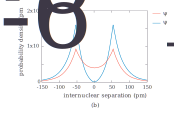
\includegraphics[width=0.5\textwidth]{10.4.1-b.pdf}
	\caption{}
	\label{fig:10.4.1}
\end{figure}
To find the wavefunction of a molecule in a given state/orbital, we apply the linear combination of atomic orbitals approximation, which can be generally written as,
\begin{equation}
	\psi_i(\vb{r}_e) = \sum_m c_m^i\psi_m(\vb{r}_m)
\end{equation}
where $\psi_m$ are atomic orbitals located at nuclear position $\vb{a}_m$ with $\vb{r}_m = \vb{r}_e - \vb{a}_m$.
\\\\
Let's consider the H$_2^+$ ion specifically, whose wavefunction is given by a linear combination of $1s$ orbitals,
\begin{equation}
	\psi^{\pm}(\vb{r}_e) = N_{\pm} \left[\psi_a(\vb{r}_a)\pm\psi_b(\vb{r}_b)\right]
\end{equation}
where $N_{\pm}$ is a normalisation constant. If we analyse the probability density $\abs{\psi^{\pm}}^2$, like in figure \ref{fig:10.4.1}. We can see that in the even $\psi^+$ state the proton has a high probability being between the two protons, and can bind the protons due to the Coulomb attraction, and thus is known as a \textbf{binding orbital}. The odd $\psi^-$ state is known as the \textit{antibonding orbital}, as in this state it will not bind the protons together.
\section{Energy Expectation of H$_2^+$}
The Hamiltonian of the H$_2^+$ ion is,
\begin{equation}
	\hat{H} = -\frac{\hbar^2}{2m_e}\laplacian_e -\frac{e^2}{4\pi \epsilon_0 r_a} -\frac{e^2}{4\pi \epsilon_0 r_b} + \frac{e^2}{4\pi \epsilon_0 r}.
\end{equation}
We can then write the expectation value,
\begin{equation}
	E^{\pm} = \frac{\int(\psi^{\pm})^*\hat{H}\psi^{\pm}\dd{\vb{r}}_e}{\int\abs{\psi^{\pm}}^2\dd{\vb{r}_e}} = \frac{H \pm H_{ab}}{1 \pm S}
\end{equation}
where,
\begin{align}
	H & = H_{aa} = H_{bb} = \int\psi_a^*\hat{H}\psi_a\dd{\vb{r}_e} = \int\psi_b^*\hat{H}\psi_b\dd{\vb{r}_e} \\
	H_{ab} & = \int\psi_a^*\hat{H}\psi_b \dd\vb{r}_e \\
	S & = \int\psi_a^*\psi_b\dd{\vb{r}_e}.
\end{align}
Evaluating these,
\begin{align}
	H & = E_{1s} + \frac{e^2}{4\pi\epsilon_0r} + C \\
	H_{ab} & = \left(E_{1s} + \frac{e^2}{4\pi\epsilon_0r}\right)S + K
\end{align}
where 
\begin{align}
	C & = \int\psi^*_a\left(-\frac{e^2}{4\pi\epsilon_0r_b}\right)\psi_a \dd{\vb{r}_e} \\
	K & = \int\psi_a^*\left(-\frac{e^2}{4\pi\epsilon_0r_b}\right)\psi_b\dd{\vb{r}}_e
\end{align}
and thus,
\begin{equation}
	E^{\pm} = E_{1s} + \frac{e^2}{4\pi\epsilon_0r} + \frac{C\pm K}{1\pm S}.
\end{equation}
\begin{figure}[h]
	\centering
	\includegraphics[width=0.5\textwidth]{mol.jpg}
	\caption{Occupation level diagram for H$_2$.}
	\label{fig:mol}
\end{figure}

\chapter{Electrons in Periodical Potential}
\section{Free Electron Model of Metals}
\begin{figure}[h]
	\centering
	\includegraphics[width=0.5\textwidth]{freeelectron.png}
	\caption{}
	\label{eq:free}
\end{figure}
We will consider a one-dimensional lattice consisting of many-atoms. We will consider the electrons moving in a 1-dimensional potential due to ions of crystal. The approximate potential for a crystal of size $L$ is shown in figure \ref{eq:free}. 
\\\\
In the free electron model, we assume the particle in a box model, where the potential and corresponding solutions are,
\begin{align}
	V(x) = \begin{cases}
		0 & 0 \leq x \leq L \\
		\infty & \text{Otherwise}
	\end{cases}
	&& \psi_n(x) = \sqrt{\frac{2}{L}}\sin\frac{n\pi x}{L}
\end{align}
and the energy is given by,
\begin{equation}
	E_n = \frac{\hbar^2k^2}{2m} = \frac{\pi^2n^2\hbar^2}{2mL^2}.
\end{equation}
For a realistic crystal with $10^23$ atoms, the energy levels can be treated as being continuous spectrum $E_k$. 
\subsection{Periodic Boundary Conditions}
When dealing with the movement of electrons within a macroscopic solid, it is useful for us to implement \textit{periodic boundary conditions}:
\begin{enumerate}
	\item Assume an infinite solid, and divide it into boxes of length $L$, and assume the wavefunction is periodic such that,
	\begin{equation}
		\psi(x+L) = \psi(x).
	\end{equation}
	\item For a particle in a box, the solutions are,
	\begin{equation}
		\psi(x) = Ae^{ikx}
	\end{equation}
	and the PBC requires,
	\begin{equation}
		k = \frac{2\pi n}{L}, \hspace{2em} 	n=0,\pm1,\pm2,\ldots
	\end{equation}
\end{enumerate}
The wavevector $k$ defines the $k$-space. Each state labelled by a quantum number $n$ occupies a volume element in $k$ space of size $\frac{2\pi}{L}$. If we assume a 1D solid lattice, with $N$ cells and a lattice spacing of $a$ such that $L = Na$, there exists the \textit{first Brillouin zone} (FBZ),
\begin{equation}
	-\frac{\pi}{a} \leq k \leq \frac{\pi}{a}
\end{equation}
where there are $N$ states. I.e., the number of states within the FBZ is equal to the number of cells. 
\begin{figure}[h]
	\centering
	\includegraphics[width=0.5\textwidth]{freeeee.png}
	\caption{}
	\label{fig:freeeee}
\end{figure}
The ground state configuration of an $N$-electron solid consisting of $N$ cells is visualised in figure \ref{fig:freeeee}. Each electron can occupy up tot the Fermi momentum $k_f = \frac{\pi}{2a}$, and each state can accommodate 2 electrons, one $\uparrow$ and one $\downarrow$. The total ground sate energy is given by,
\begin{equation}
	E_g = \frac{L}{2\pi}\int_{-k_f}^{k_f} \dd{k}\cdot \frac{\hbar^2k^2}{2m_e}.
\end{equation}
\section{Bloch Theorem}
\begin{figure}[h]
	\centering
	\includegraphics[width=0.5\textwidth]{lattice.png}
	\caption{}
	\label{fig:lattice}
\end{figure}
We have previously ignored the effect of the lattice ion cores. We now want to include the effects of a lattice ion potential. This potential is visualised in figure \ref{fig:lattice}. We will attempt to guess the form of the wavefunction to be,
\begin{equation}
	\psi_k(x) = e^{ikx}u_k(x) \label{eq:bloch}
\end{equation}
where $u_k(x)$ has a periodic property,
\begin{equation}
	u_k(x+a) = u_k(x).
\end{equation}
The result of equation \eqref{eq:bloch} is the \textit{Bloch Theorem}.
\begin{Theorems}{Bloch Theorem}
	The eigenfunctions of the wave equation for a periodic potential are the product of a plane wave $\exp(ikx)$ times a function $u_k(x)$ with the periodicity of the crystal lattice. 
\end{Theorems}
We can then derive the following condition,
\begin{equation}
	\psi_k(x + a) = e^{ika}\psi_k(x)
\end{equation}
\section{Kronig-Penny Model of Solids}

\appendix
\chapter{Misc. Formulae}
\section{Commutation Relation}
\begin{align}
	\left[\hat{A}\hat{B}, \hat{C}\right] = \left[\hat{A}, \hat{C}\right]\hat{B} + \hat{A}\left[\hat{B},\hat{C}\right] \\
	\left[\hat{A} + \hat{B}, \hat{C}\right] = \left[\hat{A}, \hat{C}\right] + \left[\hat{B},\hat{C}\right]
\end{align}
\section{Legendre Polynomials}
Legendre polynomials follow the orthogonality relation,
\begin{equation}
	\int_{-1}^1 P_l(x)P_m(x) = \frac{2}{2l+1}\delta_{lm}
\end{equation}
and associated Legendre polynomials follow,
\begin{equation}
	\int_{-1}^1 P_k^mP_l^m = \frac{2(l+m)!}{(2l+1)(l-m)!}\delta_{kl}.
\end{equation}
\end{document}
